\chapter{Applications Of The Forward Problem}

The ECG is the first tool cardiac physicians turn to when diagnosis of a problem is
required.
A model of the atria and the surface potentials developed by the excitation of
the model can be used to correlate ECG profiles to cardiac function in a variety
of conditions.
This can provide more details about the direct link between ECG indices and
cardiac arrhythmia or other dysfunction.

While inverse solutions promise to reproduce the excitation sequence of the
heart from the recorded potentials on the surface, the technique has serious
limitations.
For accurate solutions, patient specific geometries have to be constructed from
MRI scans.
There is also a need for complex lead systems, sometimes featuring more than two
hundred leads.
Also, many of the inverse techniques rely on `smooth' propagation patterns to
reduce the uncertainties in the technique which may not be found in pathological
cases.
A device which can perform such calculations automatically is a long way off,
both in terms of computational power required and complexities to resolve.

By contrast, diagnostic guides based on a forward solution can be of use to any
doctor.
They can also be used to further validate simulation studies of genetic or
diseased conditions, by comparison of the generated ECGs with those recorded
from real patients.
This chapter explores some of these predictions, using the model developed in
the previous chapter.



\section{Focal Atrial Tachycardia}

Atrial Tachycardias are one of the rarer forms of supraventricular
tachycardia.
They account for approximately 10\% of diagnosed supraventricular tachycardias
and tend to occur as a result of other cardiac or respiratory diseases.
They are characterised by a high heart rate ($\leq$ \unit{250}{bpm}) and
typically have evidence of an abnormal cardiac axis or P-wave
morphology~\cite{MacFarlaneSinus1989}.
They are hard to treat with drugs, but radiofrequency ablation can be used with
a high probability of success.
Diagnosis of atrial tachycardia, and focus, can be difficult due to a lack of
research data.
Attempts to locate the sites of the ectopic focus are current topics of clinical
research~\cite{Kistler2006,Kahn2006,Yamane2001}.
In this part of the study, I investigated possible correlations between P-wave
ECG profiles and variation in ectopic focal site.

\subsection{Model of Focal Atrial Tachycardia}

To simulate focal atrial tachycardia, the model developed in Chapter 4 was used.
The model was paced from a number of sites located around the atria, close to
common foci of focal point tachycardia.
The sinus node of the model was not stimulated.
These sites are shown in figure~\ref{fig:forward:fat:sites}.
Their anatomic locations are summarised in table~\ref{tbl:forward:fat:sites}.
All the nodes which have active cells within 10 cells (\mm{3.3}) are excited via
direct current injection of \unit{2}{nS}\ for \ms{2}.
The resulting excitation wave is then allowed to propagate without interference
and the BSPM, ECG and derived VECG calculated.
The algorithm developed by Kistler~et~al.~\cite{Kistler2006}\ is applied to the
12 lead ECG and the origin of the focal point tachycardia estimated.

\begin{figure}
\begin{center}
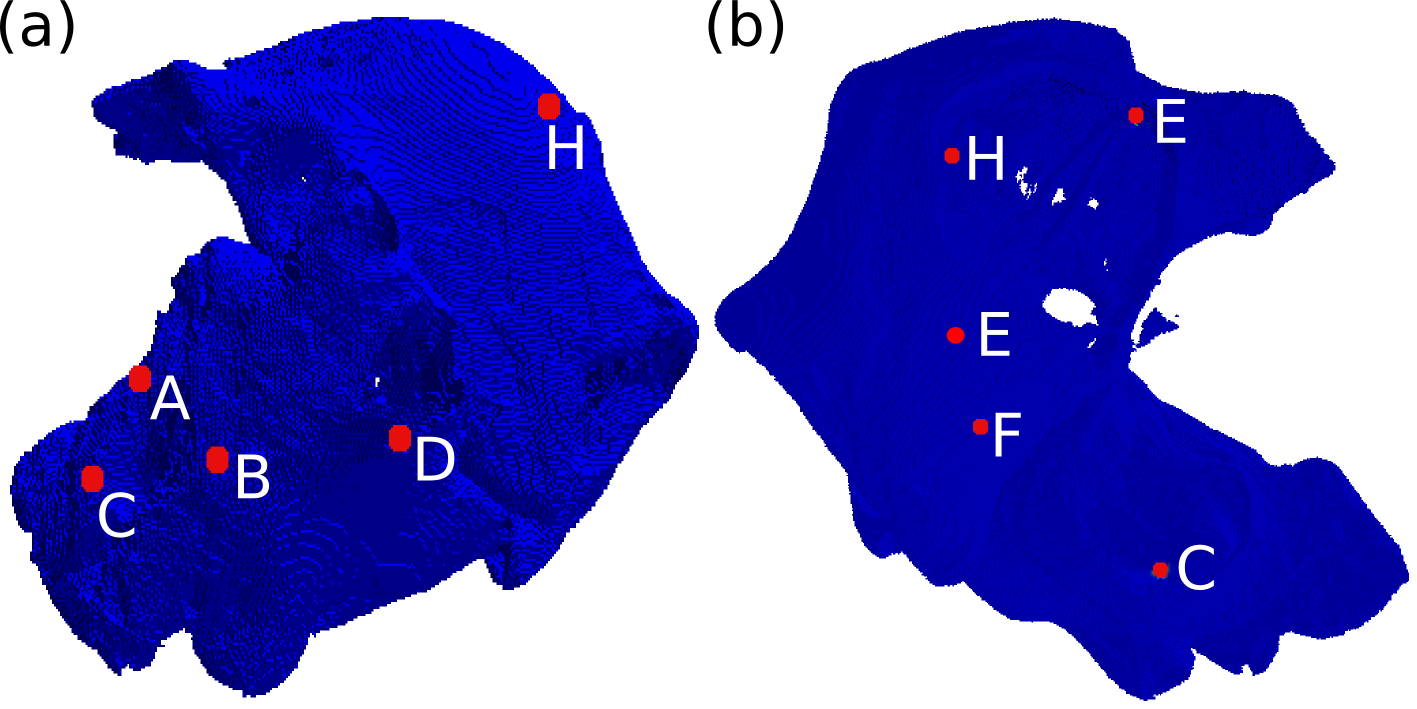
\includegraphics{figures/forward/kistler/pacing_sites}
\end{center}
\caption[Pacing Sites Around The Atria]{
\label{fig:forward:fat:sites}
Pacing sites used assessment of the Kistler~et~al. algorithm.
The pacing centres are indicated by red dots.
Note that sites are often on the interior of the atria at the indicated
locations, or embedded in the wall.

(a) View of the pulmonary veins.
(b) View of up through the valve openings.
}
\end{figure}

\begin{table}
\caption[Pacing Sites Around The Atria]{
\label{tbl:forward:fat:sites}
Anatomical locations of the pacing sites chosen for the study.
Abbreviations: AA = atrial appended, PV = pulmonary vein, TA = tricuspid anulus,
CS = coronary sinus, S = septum, CT = crista terminalis.
L and R denote left and right, respectively.
}
\begin{center}
\begin{tabular}{l l}
\toprule
Site &  Origin \\
\midrule
A & LPV \\
B & LPV \\
C & LPV \\
D & RPV \\
E & RAA \\
F & CS \\
G & LS \\
H & CT \\
\bottomrule
\end{tabular}
\end{center}
\end{table}
\subsection{Results}

\subsubsection{Twelve Lead ECG}

Pacing the atria from different sites results in a dramatic variability in the
observed waveforms of the P-wave ECG.
The ECGs corresponding to the stimuli are shown in
figure~\ref{fig:forward:fat:ecgs}.
The classifications of the waveforms are shown in
table~\ref{tbl:forward:fat:ecgs}.
Classifications consider only the P-wave and not the $\text{T}_{\text{P}}$
wave.
In the case of more than two significant deflections, the largest two are
chosen.
The effect of any electrical flow is exaggerated by the large P-wave magnitudes
previously noted and so it is likely that with correct magnitudes in the
P-waves, these lesser deflections would not show.


\begin{figure}
\begin{center}
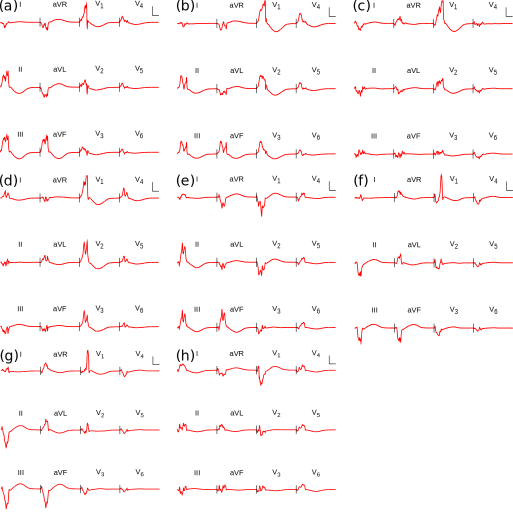
\includegraphics{figures/forward/kistler/ecgs}
\end{center}
\caption[P-wave ECGs For Ectopic Focal Sites]{
\label{fig:forward:fat:ecgs}
Shown is one complete P-wave and $\text{T}_{\text{P}}$ wave, associated with
each of the pacing sites A--H (table~\ref{tbl:forward:fat:sites}).
Scalebars are shown for each figure.
The vertical scale bar is \mv{0.2}, the horizontal \ms{100}.
}

\end{figure}

\begin{table}
\caption[Lead classification from pacing sites through the atria]{
\label{tbl:forward:fat:ecgs}
Lead classification after pacing from sites along the crista terminalis.
Leads are classified based on the criteria used by
Kistler~et~al.~\cite{Kistler2006}.
A positive P-wave is denoted by a $+$ sign, a negative P-wave by a $-$ sign and
a isoelectric (no significant positive or negative component) one by $\sim$.
In the case of a biphasic wave, it is classified based on the polarity of the
two component waves, separated by a slash.
Site denotes the pacing site as illustrated in figure~\ref{fig:forward:fat:sites}.
Site S denotes pacing from the sinus node, and is provided for comparison.
}
\begin{center}
\begin{tabular}{c c c c c c c c c c c c c}
\toprule
Site & I & II & III & aVR & aVL & aVF & $\text{V}_{\text{1}}$ &$\text{V}_{\text{2}}$ & $\text{V}_{\text{3}}$ & $\text{V}_{\text{4}}$ & $\text{V}_{\text{5}}$ & $\text{V}_{\text{6}}$\\
\midrule
S & $+$ & $+$ & $+$ & $-$ & $-$ & $+$ & $+/-$ & $+/-$ & $+$ & $+$ & $+$ & $+$ \\
A & $-$ & $+$ & $+$ & $-$ & $-$ & $+$ & $+/-$ & $+$ & $+$ & $+$ & $+$ & $+$ \\
B & $-$ & $+$ & $+$ & $-$ & $-$ & $+$ & $+$ & $+$ & $+$ & $+$ & $+$ & $+$ \\
C & $\sim$ & $-$ & $\sim$ & $+$ & $\sim$ & $\sim$ & $+$ & $+$ & $+$ & $-$ & $-$ & $-$ \\
D & $+$ & $\sim$ & $-$ & $-$ & $+$ & $-$ & $+$ & $+$ & $+$ & $+$ & $+$ & $+$ \\
E & $+$ & $+$ & $+$ & $-$ & $-$ & $+$ & $-$ & $-$ & $\sim$ & $+$ & $+$ & $+$ \\
F & $+/-$ & $-$ & $-$ & $+$ & $+$ & $-$ & $-/+$ & $-/+$ & $-$ & $-$ & $-$ & $-$ \\
G & $+$ & $-$ & $-$ & $+$ & $+$ & $-$ & $\sim/+$ & $-/+$ & $-$ & $-$ & $-$ & $-$ \\
H & $+$ & $+$ & $-/+$ & $-$ & $+$ & $+$ & $+/-$ & $+/-$ & $+$ & $+$ & $+$ & $+$ \\
\bottomrule
\end{tabular}
\end{center}
\end{table}

Pacing from site A, shown in figure~\ref{fig:forward:fat:ecgs}(a), results in a
P-wave which is positive in most leads.
The P-wave is positive in leads II, III, aVF and $\text{V}_{\text{1--6}}$.
It is negative in leads I, aVR and aVL.
The sharp negative spike visible in $\text{V}_{\text{1, 2}}$ at approximately
\ms{110}\ is caused by the faster conduction along the pectinate muscles, which
are in places disconnected from the main wall of the atrium.
This causes brief high voltage `islands' to appear ahead of the main wavefront,
which generate dipoles of opposing sign to the main wavefront.
This isn't a problem under sinus rhythm, which shows a much more regular
excitation of the pectinate muscles due to the differing origin of excitation.
In addition, the exication wave front has just started to loop back around the
inferior vena cava, travelling away from the frontal precordial leads.
Many of the limb leads show a quite ragged profile, and are slightly bifid.

Pacing from site B, shown in figure~\ref{fig:forward:fat:ecgs}(b), results in a
P-wave which is positive in most leads.
The P-wave is positive in leads II, III, aVF and $\text{V}_{\text{1--6}}$.
It is negative in leads I, aVR and aVL.
All of the inferior leads (II, III and aVF) are smooth but highly bifid.
This occurs as the P-wave depolarises first down the left atrium and then the
right, away from the left limb lead electrode.
After the initial depolarisation of the left atrium from the top and right,
towards the left, much of the excitory activity is parallel to the lateral
precordial leads ($\text{V}_{\text{4--6}}$).

Pacing from site C, shown in figure~\ref{fig:forward:fat:ecgs}(c), results in a
P-wave which is relatively flat.
The P-wave is positive in aVR and $\text{V}_{\text{1--3}}$.
It is negative in leads II and $\text{V}_{\text{4--6}}$.
It is biphasic in leads I, III, aVL, aVF.
The signal in all leads, though especially III, aVF and $\text{V}_{\text{4}}$ is
highly variable.
This is due to an uneven propagating wavefront, caused by the anatomical
obstacles.

Pacing from site D, shown in figure~\ref{fig:forward:fat:ecgs}(d), results in a
P-wave which is mostly positive.
The P-wave is positive in leads I, aVL and $\text{V}_{\text{1--6}}$.
It is clearly bifid in all the leads it is positive in, except lead
$\text{V}_{\text{1}}$.
The P-wave is negative in leads III, aVR and aVF.
It is bifid in both III and aVR.
The ECG is biphasic in lead II.

Site E is shown in figure~\ref{fig:forward:fat:ecgs}(e).
The P-wave is positive in lead I, II, III, AVF and $\text{V}_{\text{5, 6}}$.
The P-wave is negative in lead aVR, aVL and $\text{V}_{\text{1--3}}$.
The P-wave is biphasic in lead $\text{V}_{\text{4}}$.
It is bifid in the positive leads II, III and aVF and in the negative leads aVR,
aVL and $\text{V}_{\text{1, 2}}$.
The P-wave is smooth in most leads, aside from the bifidity.
The electrical excitation is spreading down and slightly to the left of the
body, leading to the very positive potentials observed in the inferior leads,
and the positive potentials in leads $\text{V}_{\text{4--6}}$.
The negative potentials in leads $\text{V}_{\text{1, 2}}$ suggest a spread of
excitation anterior to posterior.

Pacing from site F, figure~\ref{fig:forward:fat:ecgs}(f), produces predominately
negative P-waves.
The P-wave is positive in leads aVR and aVL.
It is negative in leads II, III, aVT and $\text{V}_{\text{3--6}}$.
It is biphasic in leads I, $\text{V}_{\text{1}}$ and $\text{V}_{\text{2}}$.
The P-wave is generally quite clean in all the leads, although it shows
significant oscillation at the end of the P-wave in leads II, III and aVF.
This is likely causes as the excitation wave which is spreading up the right
atrium encounters the complex anisotropy of the junctions between the crista
terminalis and the pectinate muscles.


Pacing from site G, shown in figure~\ref{fig:forward:fat:ecgs}(g), produces a
predominately negative P-wave.
The P-wave is positive in leads I, aVR and aVL.
It is negative in leads II, III, aVF and leads $\text{V}_{\text{3--6}}$.
It is biphasic in leads $\text{V}_{\text{1}}$ and $\text{V}_{\text{2}}$.
The negative leads $\text{V}_{\text{3--6}}$ are indicative of a left atrial
pacing site, with the excitation mostly spreading away from the left.
The positive P-wave in leads aVR and aVL, combined with the negative P-waves in
leads II, III and aVF, suggest the excitation is at the base of the heart and is
spreading upwards.
The lead traces are generally clean.

Site H, figure~\ref{fig:forward:fat:ecgs}(h), produces jagged P-waves.
The P-wave is positive in leads I, II, aVL and $\text{V}_{\text{4--6}}$.
The P-wave is negative in lead aVR.
The P-wave is $-/+$ biphasic in leads III, aVF and $\text{V}_{\text{3}}$.
It is $+/-$ biphasic in leads $\text{V}_{\text{1}}$ and $\text{V}_{\text{2}}$.
Leads II, $\text{V}_{\text{4}}$ and $\text{V}_{\text{5}}$ are bifid.
In addition, leads aVF and $\text{V}_{\text{3}}$ are very bifid in appearance,
although the trough becomes negative enough to classify them as biphasic.

\subsubsection{Application of the Focus Location Algorithm}

The algorithm developed by Kistler~et~al. was applied to the P-wave morphologies
generated by the model.
The algorithm is presented as a simple decision tree, initially concerning the
morphology of lead $\text{V}_{\text{1}}$.
The results of applying the algorithm and the actual anatomical locations are
shown in table~\ref{tbl:forward:fat:kistler}.


\begin{table}
\caption[Classification of focal point tachycardia]{
\label{tbl:forward:fat:kistler}
Classification of the origin of focal point tachycardia according to the
algorithm developed by Kistler~et~al. compared with the actual anatomic
location.
Where the algorithm presents multiple sites as a possibility, both are given.
Abbreviations: AA = atrial appended, PV = pulmonary vein, TA = tricuspid anulus,
CS = coronary sinus, S = septum, CT = crista terminalis.
L and R denote left and right, respectively.
}
\begin{center}
\begin{tabular}{l l l}
\toprule
Site & Predicted  & Origin \\
\midrule
A & CT & LPV \\
B & LAA / LPV & LPV \\
C & RPV & LPV \\
D & RPV & RPV \\
E & RAA / TA & RAA \\
F & CS os / LS & CS \\
G & CS os/ LS & LS \\
H & CT & CT \\
\bottomrule
\end{tabular}
\end{center}
\end{table}

\subsection{Discussion and Conclusion of Focal Atrial Tachycardia Study}

The simulation results show very good agreement with the focal tachycardia
location algorithm developed by Kistler~et~al.
The algorithm, when used on the P-wave ECGs produced by the model, correctly
estimated the origin of the focal point tachycardia in six out of the eight
cases considered.
In addition, one of the errors (case C), is only mistaking between the left and
right pulmonary veins.
This is encouraging as it acts as a validation of both the model and the
algorithm.

The study also highlights some of the limitations of the model.
The most significant of these is the large amplitudes of the P-waves, due to the
nature of the inhomogeneities considered and the underlying cardiac model.
Because of this larger amplitude, several fluctuations that perhaps should be
considered minor are instead classified as full deflections due to the
\mv{0.05}\ threshold.
This is especially evident in case A which is incorrectly classified by the
algorithm as originating from the crista terminalis.
This is due to the presence of the negative spike in lead $\text{V}_{\text{1}}$.
The spike has a magnitude of approximately \mv{0.1} which causes the lead to be
classified as having a positive--negative morphology.
The algorithm classifies all such P-waves as having a crista terminalis origin.
If the spike were of a reduced amplitude, the positive $\text{V}_{\text{1}}$ and
other lead morphologies leads to a classification of LAA or LPV, the correct
answer.

It is also possible that the size of the stimulus zone should be decreased.
The effect of the localised and very rapid potential change along the border of
the stimulus zone can generate a large spike at the start of the pacing cycle.
This is due to the rapid ($ > 200\,\text{mVs}^{\text{-1}}$) upstroke of the
Courtemanche~et~al myocyte model used as the basis of the anatomical atrial
model.
A smaller stimulus zone should reduce this artefact, which is sometimes
difficult to separate from the `real' P-wave.

It should be emphasised, however, that the large amplitudes of the P-wave was
only an issue in case A.
The location of the focal point tachycardia was correctly predicted by the
algorithm in most cases.
This prediction would not be affected by a reduction in amplitude of all the
lead potentials.
The model therefore correctly reproduces the phase information of the P-wave
ECG, which is ultimately what the location algorithm depends on.

The Kistler~et~al. algorithm appears to be the best algorithm one is aware of in
the literature that uses the standard twelve lead ECG.
It would be interesting to compare the predictive accuracy of the algorithm with
one devised using the model and the so called `Atrial ECG' proposed by
Ihara~et~al~\cite{Ihara2007}.
Such a study would require a family of similar models to be developed, based on
several torso and atrial geometrical models.

No discussion of an algorithm of this nature would be complete without a
discussion of inverse techniques.
Inverse techniques have developed considerably over the previous two decades.
Ramanathan~et~al.~\cite{Ramanathan2006}\ have developed a technique which they
call Electrocardiographic Imaging (ECGI) and several groups have similar efforts
as well.
These techniques allow calculation of the epicardial potentials from external
measurements.
These inverse techniques require a significant amount of effort to set up,
however.
The ECGI techinique proposed by Ramanathan~et~al. uses a 224 electrode vest and
requires the construction of a heart--torso geometry from CT scans.
By contrast, algorithms devised for twelve lead sets can still be highly
accurate and are available everywhere.

The Kistler~et~al. model can correctly predict the location of ecotopic foci in
the body surface potential model in seven of eight cases.
This validates both the algorithm and the model.
The model could therefore be used as the basis for further refinements to the
algorithm, or the development of similar ones.

\section{Inverted P-Waves at Night}

Recently an observation was made concerning patients under
24 hour ECG monitoring (Prof. Mark Boyett, Private Conversation, 2008).
It was noted that some patients exhibited inverted P-waves at night.
That is to say, if the patient showed a positive P-wave in leads II and aVF
during the day, then at night the P-wave would be negative in leads II and aVF.
These patients had no known heart disease or conduction defects.
This phenomena has not been reported in the literature.

There is evidence~\cite{Shibata2001,Boineau1988,Dobrzynski2005} that the pacemaker is not a
small and discrete area of the atrium, but is instead distributed along the
length of the crista terminalis.
The presence of certain drugs and hormones, most notably acetylcholine, can cause
the site of the leading pacemaker to move down the pace maker complex.
Acetylcholine is released by what is know as increased `vagal tone'.
This has been observed to happen at night.

The underlying mechanisms for the inverted P-waves at night are unknown.
It was hypothesised that a pacemaker shift induced by increased vagal tone
might lead to the observed P-wave inversion.
In this study, I attempt to verify the hypothesis using the P-wave ECG model.


\subsection{Methods}

In the absence of a model for the distributed pacemaker complex in the human
heart, the direct effects of acetylcholine could not be investigated.
Instead, using the model presented in the previous chapter, several sites were
located along the crista terminalis.
These sites had a radius of 10 nodes (or approximately \mm{3.3}--although this
varied depending on the thickness of the atrial wall at the pacing site), and
therefore were approximately the same size as the sino-atrial node.
These sites are shown in figure~\ref{fig:forward:inverse:ct_sites}.
Each of these sites was stimulated via the same protocol used to stimulate the
sinus node in the original model and then the electrical excitation waves were
allowed to propagate without interference.

\begin{figure}
\begin{center}
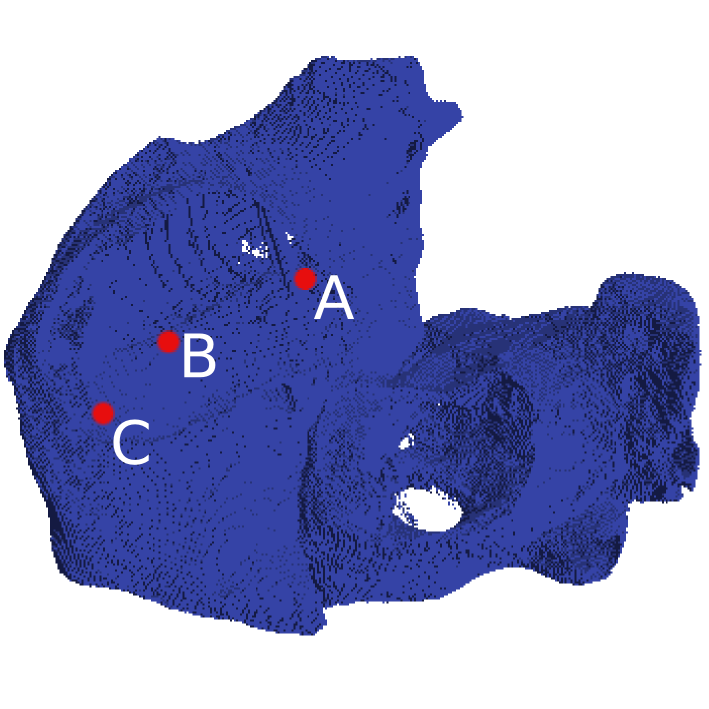
\includegraphics{figures/forward/inverted_p_wave/pacing_sites}
\end{center}
\caption[Pacing Sites Along The CT]{
\label{fig:forward:inverse:ct_sites}
Pacing sites used for the inverted P-wave study.
The view is up through the valve openings.
The pacing centres are indicated by red dots.
}
\end{figure}

The total activation time is calculated as the time after stimulus for all cells
to become excited above \mv{-60}.
ECGs were computed from the patterns of electrical excitation in the atrium.
These were compared to the sinus rhythm ECGs computed in the previous chapter.
In addition, using a so called `inverse Dower' method after Edenbrandt and
Pahlm~\cite{Edenbrandt1988}, the orthogonal components of the ECG were computed
and used to construct representations of the heart
vector~\cite{Frank1956,MacFarlane1989a} ECG (VECG).
To perform the inverse dower transformation, a matrix that has been optimized for
the P-wave (shown in Table~\ref{tbl:forward:idparams}) was
used~\cite{Guillem2007}.


\begin{table}
\caption[Inverse Dower Factors]{
\label{tbl:forward:idparams}
Factors to construct the Frank VECG from the standard 12 lead ECG set.
Parameters optimised to accurately reproduce the P-wave heart
vector~\cite{Guillem2007}.
Each of the 8 leads are multiplied by the given parameters to provide the
orthogonal Frank lead.
}
\begin{center}
\begin{tabular}{c c c c c c c c c}
\toprule
& $\text{V}_{\text{1}}$ &$\text{V}_{\text{2}}$ & $\text{V}_{\text{3}}$ &
$\text{V}_{\text{4}}$ & $\text{V}_{\text{5}}$ & $\text{V}_{\text{6}}$ & I & II \\
\midrule
X & $-0.266$ & $\:0.027$ &  $\:0.065$ & $\:0.131$ & $\:0.203$ & $\:0.220$ & $\:0.370$ & $-0.154$ \\
Y & $\:0.088$ &  $-0.088$ & $\:0.003$ & $\:0.042$ & $\:0.047$ & $\:0.067$ & $-0.131$ & $\:0.717$ \\
Z & $-0.319$ & $-0.198$ & $-0.167$ & $-0.099$ & $\:0.009$ & $\:0.060$ & $\:0.184$ & $\:0.114$ \\
\bottomrule
\end{tabular}
\end{center}
\end{table}

\subsection{Results}

\subsubsection{Activation Sequence}

The activation sequences of the atria after pacing from the sinus node, and the
three sites along the crista terminalis are shown in
figure~\ref{fig:forward:inverse:active}\ as isochronal colour maps.
Time goes from red, at \ms{0}, to blue, at \ms{150}.
The site of first activation obviously shifts depending on the stimulus
location.
In addition, as the stimulus site moves away from the sinus node, the time to
total activation of the atria increases.

\begin{figure}
\begin{center}
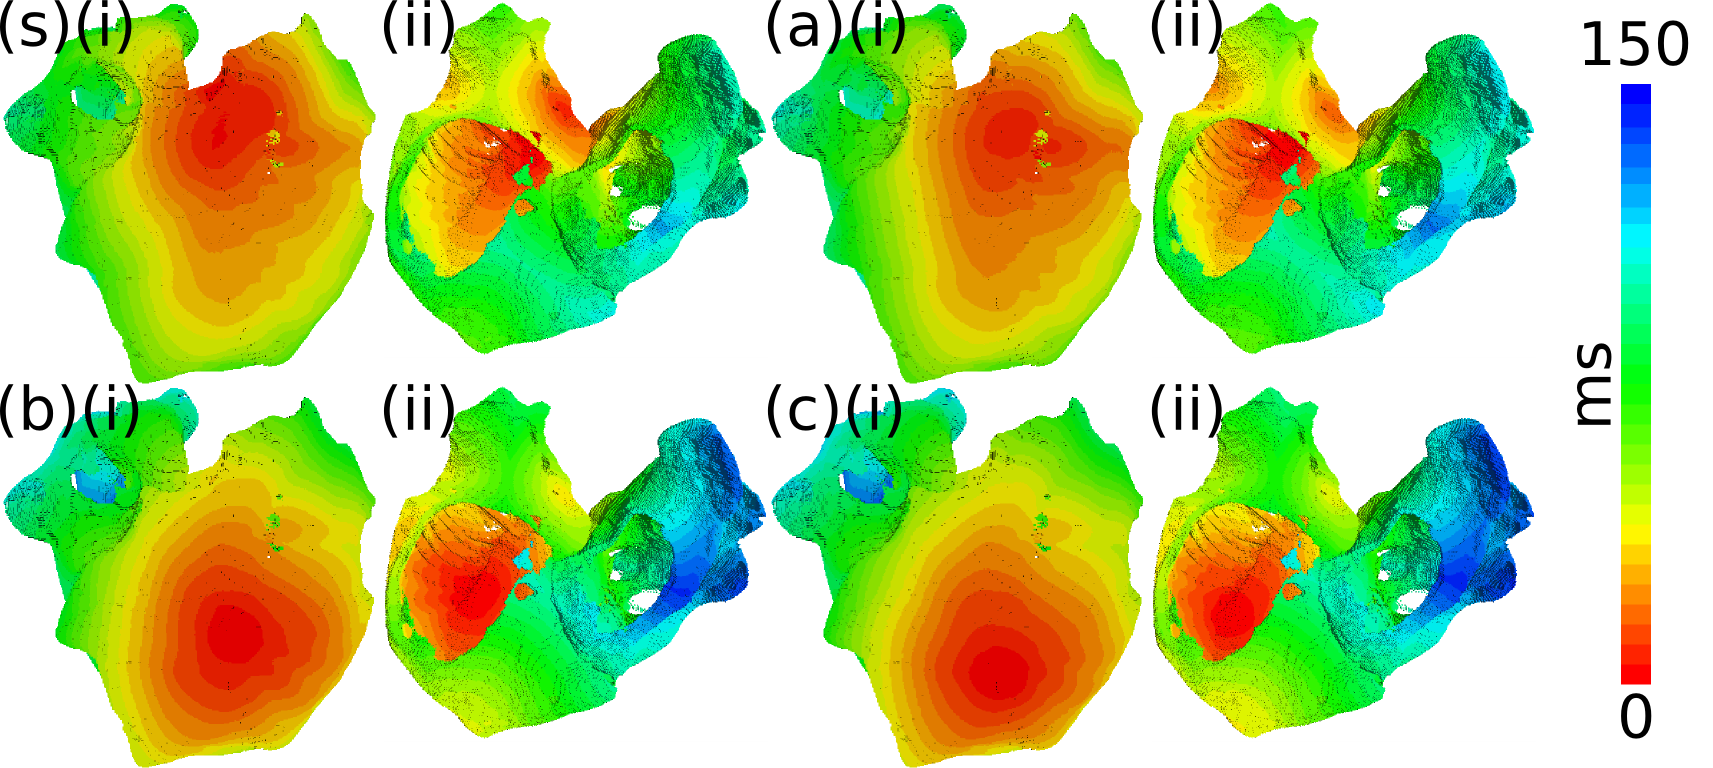
\includegraphics{figures/forward/inverted_p_wave/activation_sequence}
\end{center}
\caption[Activation sequences from pacing sites along the CT]{
\label{fig:forward:inverse:active}
Atrial activation sequences obtained from different pacing sites.
Shown are the activation sequences resulting from pacing at the sinus node, (s),
and the three crista terminalis sites A--C (a--c).
Activation times are represented by colours, going from red at $\leq$\ms{5}\
through green, \ms{75} to deep blue at \ms{150}.
Contours are every \ms{5}.

There are two views shown for each pacing site.
(i), a view of the right atrial surface with the superior vena cava at the top
of the right atrial surface and the tricuspid valve at the base.
In this view, the crista terminalis runs approximately vertically.
(ii), a view up into the atrial cavities through the valve openings.
The ribbed structures of the pectinate muscles are visible through the tricuspid
valve as they extend off the crista terminalis on the left of the panel.
The right and left atrial appendages are to the top of the panels.

In panel (s) the sinus rhythm activation sequence is visible with rapid
conduction along the crista terminalis and pectinate muscles.
The Bachmann's bundle meanwhile rapidly conducts the excitation to the left
atrium.
In both atria, the appendages are amongst the last regions to depolarise.

In panel (a), the activation sequence has shifted slightly down the crista
terminalis.
The pectinate muscles and crista terminalis still have a large influence on the
propagation.
In both atria, the appendages are the last regions to depolarise.

In panel (b), the activation sequence is shifted a long way down the crista
terminalis.
The Bachmann's bundle is no longer the site of first activation of the left
atrium.
Total time to activate is noticeably delayed.

In panel (c), the activation sequence is shifted a long way down the crista
terminalis.
Total time to activate is noticeably delayed in the left atrium.
The Bachmann's bundle is no longer the site of first activation, instead the
area close to the coronary sinus is first activated.
}
\end{figure}

The sinus node activation sequence,
figure~\ref{fig:forward:inverse:active}(s)(i, ii), starts high on the right
atrium, close to the superior vena cava.
Conduction is especially rapid down the crista terminalis and along the
pectinate muscles, visible as the more widely spaced isochrones along these
structures.
The Bachmann bundle, meanwhile, conducts the electrical excitation to the left
atrium, where it then starts to spread over the left atrial endocardial surface.
In the right atrium the activation finishes, approximately \ms{80}\ after
stimulation started, with the activation of the ring around the tricuspid valve
and the right atrial appendage.
In the left atrium, the far extremities of the left atrial appendage and the far
side of the mitral valve to the Bachmann bundle are activated at approximately
\ms{120}, completing the activation of the atria.

The activation sequence from site A,
figure~\ref{fig:forward:inverse:active}(a)(i, ii), starts high on the right
atrium in the region where the pectinate muscles are branching from the crista
terminalis.
This leads to rapid conduction down the pectinate muscles and in both directions
along the crista terminalis.
The Bachmann bundle conducts the excitation to the left atrium, where it starts
to spread.
The activation of the right atrium finishes with the activation of the right
atrial appendage and then region between the septum and the tricuspid valve.
Activation of the left atrium completes in \ms{132}\ after the initial stimulus
on the edge of the left atrial appendage and the mitral valve.

Pacing from site B leads to the activation sequence depicted in
figure~\ref{fig:forward:inverse:active}(b)(i, ii).
The activation sequence starts lower on the crista terminalis, and is conducted
in both directions along the muscle ridge.
The pectinate muscles also influence the conduction, although the excitation
wavefront reaches them later.
Excitation still reaches the left atrium through the Bachmann bundle, although
it is also conducted through the septum close to the inferior vena cava.
The last region to be excited in the right atrium is still the appendage.
In the left atrium, the last activation comes at \ms{140}.
The left atrial appendage and the sheaths of the pulmonary veins both finish
activating at this time.

The activation sequence which results from pacing from site C is shown in
figure~\ref{fig:forward:inverse:active}(c)(i, ii).
The activation sequence starts low on the right atrium and spreads in all
directions, but is faster travelling up the crista terminalis.
The pectinate muscles, when the excitation wave reaches them, also have a
noticeable effect, speeding activation of the right atrium.
Once again, the left atrium appears to be excited in two places, both by the
bachmann's bundle and close to the inferior vena cava through the septum.
The right atrial appendage is the last region of the right atrium to be excited.
In the left atrium, the extremities of the appendage and the pulmonary vein
sheaths are the last to be excited, as well as the region close to the mitral
valve.
The last activation comes at \ms{144}.

All of the activation sequences are approximately normal, in that they travel
from right to left.
The further the stimulus site is removed from the sinus node, the longer
excitation tends to take.


\subsubsection{Twelve Lead ECG}

The ECGs from the three pacing locations along the CT are shown in
figure~\ref{fig:forward:inverse:ecgs}\ with the sinus rhythm P-wave ECG for
comparison.
A summary of the lead deflections for the four cases and sinus rhythm are
presented in table~\ref{tbl:forward:inverse:ecgs}.
There is a clear evolution of the P-wave morphology visible as the pacing site
is moved down the crista terminalis.

\begin{table}
\caption[Lead classification from pacing sites along the CT]{
\label{tbl:forward:inverse:ecgs}
Lead classification of the P-wave after pacing from sites along the crista
terminalis.
Leads are classified based on the criteria used by
Kistler~et~al.~\cite{Kistler2006}.
A positive P-wave is denoted by a $+$ sign, a negative P-wave by a $-$ sign.
In the case of a highly bifid or biphasic wave, the signs of the two phases of
the wave are indicated on either side of a slash.
For example, $+/+$ would be a positive, bifid wave and $-/+$ would be a negative
then positive biphasic wave.
Site denotes the pacing site, where S is the sinus node and Sites A--C are as
indicated in Figure~\ref{fig:forward:ct_sites}.
}
\begin{center}
\begin{tabular}{c c c c c c c c c c c c c}
\toprule
Site & I & II & III & aVR & aVL & aVF & $\text{V}_{\text{1}}$ &$\text{V}_{\text{2}}$ & $\text{V}_{\text{3}}$ & $\text{V}_{\text{4}}$ & $\text{V}_{\text{5}}$ & $\text{V}_{\text{6}}$\\
\midrule
S   & $+$ & $+$ & $+$ & $-$ & $-$ & $+$ & $+/-$ & $+/-$ & $+$ & $+$ & $+$ & $+$ \\
A   & $+$ & $+$ & $+$ & $-$ & $-$ & $+$ & $+/-$ & $-$ & $+$ & $+$ & $+$ & $+$ \\
B   & $+$ & $+/+$ & $-/+$ & $-/-$ & $+$ & $+/+$ & $+/-$ & $+/-$ & $+/+$ & $+/+$ & $+$ & $+$ \\
C   & $+$ & $-/+$ & $-$ & $-$ & $+$ & $-/+$ & $+/-$ & $+/-$ & $-/+$ & $+$ & $+$ & $+$ \\
\bottomrule
\end{tabular}
\end{center}
\end{table}

\begin{figure}
\begin{center}
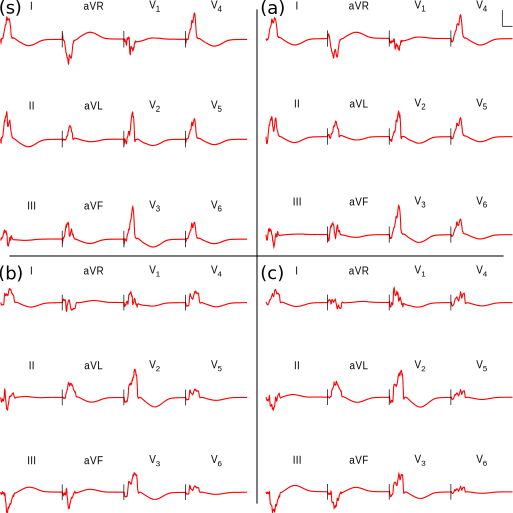
\includegraphics{figures/forward/inverted_p_wave/inverted_pwave_ecg}
\end{center}
\caption[12 Lead ECG traces from pacing sites along the CT]{
\label{fig:forward:inverse:ecgs}
Twelve lead ECG recordings obtained from the model after pacing at the sinus
node, (s) and the three pacing sites A--C (a--c).
Shown is one complete P-wave and $\text{T}_{\text{P}}$ wave, pacing at a rate of
\unit{60}{bpm}.
The scale is the same for all traces, indicated in the top right of panel (a),
where the horizontal scale is in ms and the vertical in mV.
The P-wave is positive in leads II and aVF after pacing from the sinus node.
It is positive in leads II and aVF after pacing from site A.
Pacing from site B leads to a positive but highly bifid P-wave in both leads II
and aVR.
Site C shows negative then positive biphasic P-waves in both leads II and aVR.
}
\end{figure}


The P-wave ECG for pacing from the sinus node,
figure~\ref{fig:forward:inverse:ecgs}(s), is positive in leads II and aVF.
Leads I, III and $\text{V}_{\text{3--6}}$ are also positive.
Leads aVR and aVL are negative.
Leads $\text{V}_{\text{1}}$ and $\text{V}_{\text{2}}$ are both
positive--negative biphasic.
The cardiac axis is between \degr{+60}\ and \degr{+90}\ in the frontal plane.
The ECG is consistent with a normal activation of the atria, spreading to the
left and bottom as time evolves.


Pacing from site A (figure~\ref{fig:forward:inverse:ecgs}(a)), the P-wave ECG is
positive in leads II and  aVF.
Leads I, III,  aVF and $\text{V}_{\text{3--6}}$ are also positive.
Lead aVR, aVL and $\text{V}_{\text{2}}$ are negative
Lead $\text{V}_{\text{1}}$ is posiive--negative biphasic.
The cardiac axis is between \degr{+60}\ and \degr{+90}\ in the frontal plane.
The ECG is consistent with a mostly normal propagation.
The slightly broader negative trough on lead $\text{V}_{\text{1}}$ is due to the
slightly slower depolarisation time of the left atrium.
There is a prominent notch visible in several of the limb leads.
This is caused by the depolarisation of the right atrial appendage and the
pulmonary veins, both of which happen against the bulk direction of excitation
propagation.

Pacing from site B (figure~\ref{fig:forward:inverse:ecgs}(b)), the P-wave ECG
is positive in leads II aVF, but is highly bifid.
Leads I, aVL and $\text{V}_{\text{3--6}}$ are also positive.
Lead aVR is negative.
Lead $\text{V}_{\text{1}}$ and $\text{V}_{\text{2}}$ are positive--negative
biphasic.
Lead III is negative--positive biphasic.
The cardiac axis is approximately \degr{+30} in the frontal plane.
The bifid morphology of the P-wave in the inferior limb leads and aVR is due to
the delayed depolarisation of the left atrium, induced by the time taken to
propagate up the crista terminalis.
The bidirectional propagation contributes to the much lower amplitudes observed
in many of the limb leads compared to the sinus rhythm.


Pacing from site C (figure~\ref{fig:forward:inverse:ecgs}(c)), the P-wave ECG is
negative--positive biphasic in leads II and aVR.
Leads I, aVL and $\text{V}_{\text{4--6}}$ are positive.
Leads III and aVR are negative.
Lead $\text{V}_{\text{1}}$ and $\text{V}_{\text{2}}$ are positive--negative
biphasic.
Lead $\text{V}_{\text{3}}$ is negative--positive.
biphasic.
The cardiac axis is approximately $0^\circ$ in the frontal plane, as the
excitation wave now travels mostly across the atria.
The negative--positive morphology of the P-wave in leads II and aVR are caused
as the bulk direction of the excitation is first up the right atrium and then
down the left atrium.
The lateral precordial leads ($\text{V}_{\text{4--6}}$) are positive as the
excitation is still travelling from right to left.

As the pacing site moves down the crista terminalis there is an evolution of the
P-wave, which is visible in all leads.
As a result of the shift, the cardiac axis shifts through about $90^\circ$
anti-clockwise from the sinus direction of $+90^\circ$.
The P-wave duration increases slightly as the crista terminalis increases,
highlighting the importance of the specialized conduction structures of the
heart in rapidly conducting the excitation wave.


\subsubsection{Derived Vector ECGs}

\begin{figure}
\begin{center}
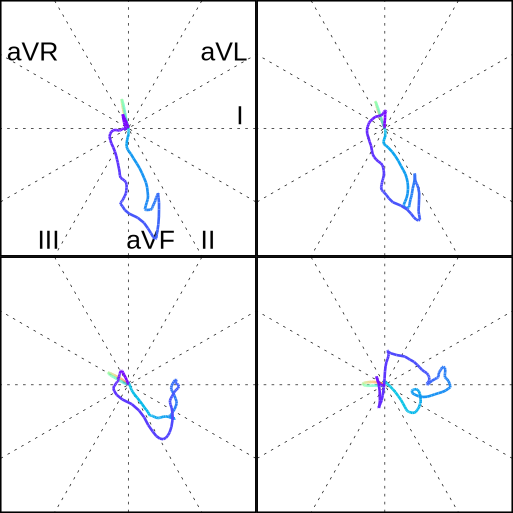
\includegraphics{figures/forward/inverted_p_wave/frontal_vector_loops}
\end{center}
\caption[Frontal plane vector loops from pacing sites along the CT]{
\label{fig:forward:inverse:vec_front}
Frontal plane vector loops, constructed from the derived vECG for pacing at the
sinus node, (s) and the three pacing sites A--C (a--c).
Shown is one complete P-wave and $\text{T}_{\text{P}}$ wave, pacing at a rate of
\unit{60}{bpm}.
Colour represents the passage of time, going from purple (\ms{0}) through blue
(\ms{250}) to red (\ms{500}) after the initiation of the stimulus.
The horizontal and vertical scales are centred at \mv{0}\ in the centre of the
figure and extending out to $\pm$\mv{0.4}.}
\end{figure}

\begin{figure}
\begin{center}
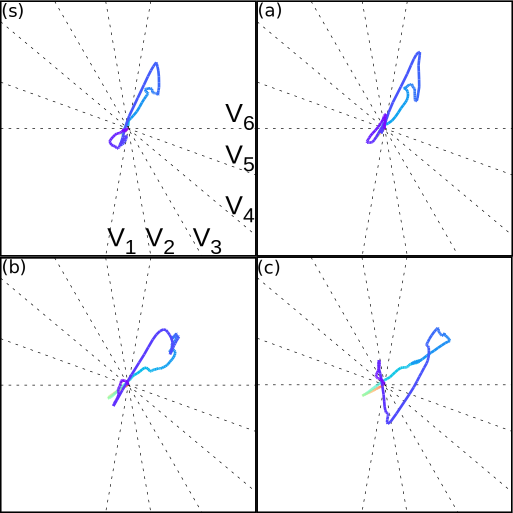
\includegraphics{figures/forward/inverted_p_wave/transverse_vector_loops}
\end{center}
\caption[Transverse plane vector loops from pacing sites along the CT]{
\label{fig:forward:inverse:vec_trans}
Transverse plane vector loops, constructed from the derived vECG for pacing at the
sinus node, (s) and the three pacing sites A--C (a--c).
Shown is one complete P-wave and $\text{T}_{\text{P}}$ wave, pacing at a rate of
\unit{60}{bpm}.
Colour represents the passage of time, going from purple (\ms{0}) through blue
(\ms{250}) to red (\ms{500}) after the initiation of the stimulus.
The horizontal and vertical scales are centred at \mv{0}\ in the centre of the
figure and extending out to $\pm$\mv{0.4}.}
\end{figure}

The derived vector ECG plots are shown for the frontal plane in
figure~\ref{fig:forward:inverse:vec_front} and in the transverse plane in
figure~\ref{fig:forward:inverse:vec_trans}.
Again, the sinus rhythm is included in both figures for reference.
The colour of the vector loop represents the passage of time and is coloured
from purple, at \ms{0}, through blue, green, yellow and ending up red at
\ms{500} after initiation of the P-wave.

The vector loop in the frontal plane for sinus rhythm is shown in
figure~\ref{fig:forward:inverse:vec_front}(s).
The vector loop is inscribed in an anti-clockwise direction.
The efferent, or outgoing, limb is at approximately \degr{+90}, before it loops up to its
maximal extension at approximately \degr{+75}.
The afferent, or incoming, limb is at approximately \degr{+70}.
The $\text{T}_{\text{P}}$ wave is visible as a small anti-clockwise loop,
almost linear, aligned at approximately \degr{-100}.
The initial deflection along almost the same line is an artefact of the stimulus
protocol.
The P-wave loop is open, although like the ECGs it is not entirely smooth.

The frontal plane vector loop for pacing from site A,
figure~\ref{fig:forward:inverse:vec_front}(a), is inscribed in an anti-clockwise
direction.
The loop is generally open, although there is a noticeable direction change
where the afferent limb briefly returns to the efferent limb.
This corresponds to the notch visible in the inferior limb leads.
The main axis of the loop is at approximately \degr{+70}.
The efferent limb is aligned at approximately \degr{+60}, along the line of lead
II.
The $\text{T}_{\text{P}}$ wave is visible as a small loop, aligned at
approximately \degr{-120}.

Pacing from site B produces the frontal plane vector loop in
figure~\ref{fig:forward:inverse:vec_front}(b).
The loop is largely inscribed in an anticlockwise direction.
The main axis of the loop is aligned at approximately \degr{+40}.
The efferent limb is relatively smooth as it travels out along an approximately
\degr{+60}\ vector.
The loop then sweeps up to \degr{+0}, crossing over itself several times, before
it returns smoothly to 0.
The $\text{T}_{\text{P}}$ is a small clockwise loop at an angle of \degr{-120}.
The loop from site C has the smallest area of the loops.

The frontal plane vector loop from pacing at site C is shown in
figure~\ref{fig:forward:inverse:vec_front}(c).
The loop is largely inscribed in as a very uneven figure-of-eight which is
initially anticlockwise and is then clockwise.
The main axis of the loop is aligned at approximately \degr{+0}.
The efferent limb is initially at \degr{+90}\ before it doubles back on itself
to sweep up at an angle of \degr{-90}.
It then sweeps down to \degr{+0}, and the point of maximal extension.
The afferent limb then sweeps back, inscribing a minor clockwise loops.
The $\text{T}_{\text{P}}$ is a small anticlockwise loop at an angle of \degr{-180}.

As the pacing site moves down the crista terminalis there are clear changes in
the morphology and principle axis of the P-wave frontal vector loop.
The axis shift which could be determined from the 12 lead ECG was clearly
highlighted.
The vector loops also show the reduction in amplitude of the P-wave as the
pacing location is moved down the crista terminalis, possibly caused by the
generally slower speed of activation.
The $\text{T}_{\text{P}}$ wave axis is opposite the main axis of the loop in all
cases.

In contrast to the frontal plane vector plots, the transverse plane plots bear
much less resemblance to the associated leads ($\text{V}_{\text{1--6}}$).
The differences manifest in both the magnitude and the direction.
This makes it hard to directly compare the transverse plane vector plots with
the cardiac activity.
The loops generated appear to be too flat and too negative in the Z (vertical)
direction, which is especially obvious in the sinus rhythm plot
(\ref{fig:forward:inverse:vec_trans}(s)).

\subsection{Discussion and Conclusions of Inverted P-wave Study}

As the stimulus site moves down the crista terminalis the patterns of electrical
activation in the atrium change noticeably.
The focal point of excitation obviously moves down the crista terminalis to
follow this.
It is also interesting to note the similarities.
Despite the shifting activation site, the right atrial appendage and the region
between the tricuspid valve and the atrial septum are always the last to
activate in the right atrium.
In the left atrium, the appendage also activates last in all cases.

As the pacing site moves away from the sinus node, the total activation time
increases.
However, total activation times remain within those observed clinically by
Lemery~et~al.~\cite{Lemery2004}\ for all three pacing locations away from the
sinus node.
The activation patterns are similar to those observed by
Boineau~et~al.~\cite{Boineau1988}\ as the pacing location moves, although the
Boineau data does not include single activations away from the sinus node.

The latter two sites (B \& C), which are low on the crista terminalis, appear to
reach the left atrium in part through a site which emerges close to the coronary
sinus~\cite{Platonov2007,Platonov2008,Markides2003,Lemery2004}.
There is no specialist inferior intra-atrial conduction pathway in the model
however.
Conduction along this lower route is therefore at the normal bulk tissue rate.
It is possible if this were treated specially in the model total activation
times would be reduced.

The ECGs generated from the model also show an evolution as the stimulus site
moves down the crista terminalis.
This change is more visible in the limb leads than in the precordial leads.
This is to be expected, as the propagation remained from right to left in all
cases, but whether it is travelling up or down the atria changes as the pacing
site does.
The P-waves in leads II and aVF is positive in during sinus rhythm, and both
gradually invert as the pacing site shifts down the crista terminalis, as
hypothesised.

As the pacing site moves away from the sinus node, the P-wave duration also
increases.
Especially for the lower crista terminalis sites (B \& C), the duration exceeds
normal P-wave limits~\cite{Lemery2004,MacFarlane1989}.
It is possible that a more detailed intra-atrial conduction system, including an
inferior pathway would reduce total conduction time, and therefore P-wave
duration in these cases.

The P-wave vector loops are similar to those observed in clinical
studies~\cite{Carlson2005,Holmqvist2007,Havmoller2007,Guillem2008}, although the typical
presentation of such loops as monochromatic does make comparison of the timing
information and direction of inscription hard.
They make it quite obvious that the cardiac axis shifts as the pacing location
does.
The morphology of the loops can be used to gain further clues, such as with the
initial rise and then fall visible in the Site B frontal vector loops.

The limitations of the body surface potential model have been discussed
previously ($\S$\ref{sec:bsp:limits}).
Of particular importance to this study is the lack of a distributed sinus node
model~\cite{Yamamoto2007,Dobrzynski2005}\ for the human atrium.
However, pacemaker shift under the influence of
acetylcholine~\cite{Shibata2001}\ has been observed in rabbits and in
humans~\cite{Opthof1988}\ so it seems plausible as a mechanism for the shifts
and associated P-wave inversions.
The use of an inverse dower matrix to obtain the frank leads rather than
directly measuring them was chosen to allow more direct comparison with clinical
data, which is often only for the standard twelve leads.
The selection of the correct transform matrix is
important~\cite{Guillem2008,Luo1991b,Hyttinen1995}\ and it is possible that the
vector loop accuracy could be improved by the use of a transformation matrix
optimised for the body surface potential model~\cite{vanOosterom2007}.
This is especially true for the Z-axis, which has the lowest correllation
coefficient of the leads~\cite{Hyttinen1995}.
Alternatively a true frank lead system, or a hybrid model could be constructed.

The hypothesis that P-wave inversion could be caused by pacemaker shift in the
human sinus node seems to be plausible.
Progressive shift of the pacemaker site down the sinus node leads to progressive
inversion of the observed P-waves in leads II and aVF.
In addition, this shift is accompanied by other changes which do not stray too
far from normality.
This is important, as the shift was originally observed in those with no
diagnosed cardiac disorders.
Further investigation is merited, once an appropriate model of the distributed
sino-atrial node complex can be integrated into the atrial model.

This study shows that the body surface potential model can be used for a study
which involves conditions that begin to deviate from normality.
It can therefore be used as a powerful tool for investigating the clinically
observable consequences of changes to cardiac behaviour.

\section{Discussion and Conclusion}

The constructed model has been used in two separate studies.
The first was a validation of an existing clinically derived algorithm for
predicting the origin of focal point tachycardia.
The second study concerned itself with investigation into a new clinical
phenomena, that of inverted P-waves at night.


The focal tachycardia algorithm study confirms the performance of the algorithm.
This validates both the algorithm and the model.
The study also highlights a potential weakness in the model, that of the high
amplitudes it produces.
Despite this problem, the model still performs well and was `well behaved'
according to the algorithm under test.
In addition, there is no indication that a reduction in the amplitude due to a
more complete consideration of the inhomogeneities would adversely impact this.

The inverted P-wave study confirms that a suggested mechanism for inverted
P-waves at night, that of pacemaker shift under increased vagal tone, is
plausible.
The ECGs calculated by the model show a clear evolution as the pacing site
shifts further down the crista terminalis.
Additional validation is is obviously required with a suitable model of a
distributed pacemaker complex.

The model developed is therefore a useful tool for cardiac modelling.
It can enhance the conclusions that can be drawn from 3D simulations with
further clinical relevance.

